\documentclass[mathserif]{beamer}
\usepackage{subfigure}
\usepackage{listings}
\usepackage{courier}
\definecolor{lightlightgray}{gray}{0.95}
\definecolor{lightlightblue}{rgb}{0.4,0.4,0.95}
\definecolor{lightlightgreen}{rgb}{0.8,1,0.8}
\lstset{language=C++,
           frame=single,
           basicstyle=\ttfamily\footnotesize,
           keywordstyle=\color{black}\textbf,
           backgroundcolor=\color{lightlightgray},
           commentstyle=\color{blue},
           frame=single
           }
\usetheme[secheader]{pecostalk}
\usepackage{bibentry}
\nobibliography*
\graphicspath{{figs/}}                                                                                                                              

% defines newblock as null, giving compile issues otherwise
\let\newblock\relax 

\newcommand{\eqdef}{\stackrel{\text{\tiny def}}{=}}

\newcommand{\NVRvect}[1]{\ensuremath\boldsymbol{#1}}
\newcommand{\vect}[1]{\ensuremath\boldsymbol{#1}}
\newcommand{\NVRtensor}[1]{\NVRvect{#1}}
%\newcommand{\NVRtensor}[1]{\underline{\NVRvect{#1}}}
\newcommand{\NVRnorm}[1]{\left|\left|#1\right|\right|}
\newcommand{\norm}[1]{\left|\left|#1\right|\right|}
\newcommand{\NVRgrad}{\nabla}
\newcommand{\NVRdiv}{\NVRgrad \cdot}
\newcommand{\NVRpd}[2]{\frac{\partial#1}{\partial#2}}
\newcommand{\NVRpdd}[2]{\frac{\partial^2#1}{\partial#2^2}}
\newcommand{\NVReqdef}{\stackrel{\text{\tiny def}}{=}}

\newcommand{\NVRHgrad}{H(\text{grad})}
\newcommand{\NVRHdiv}{H(\text{div})}
\newcommand{\NVRsumm}[2]{\ensuremath\displaystyle\sum\limits_{#1}^{#2}}
 
\newcommand{\NVRcurl}{\nabla \times}
\newcommand{\NVRHcurl}{\ensuremath H(\text{curl})}

\newcommand{\code}[1]{\texttt{#1}}
\newcommand{\deal}{\code{deal.II}\,}

\newcommand{\pecosbold}[1]{{\color{pecos2}{#1}}}
\newcommand{\pecosreallybold}[1]{{\color{pecos6}{#1}}}

\newcommand{\FootSize}{\scriptsize}

\DeclareMathOperator*{\argmin}{arg\,min}

\date{TST Meeting\\ October 17, 2012}
\author[Nate Roberts]{Nate Roberts \\
Collaborators: Leszek Demkowicz, Jesse Chan, Truman Ellis
}
\institute{Institute for Computational and Engineering Sciences\\
The University of Texas at Austin}
\title[Camellia: A DPG Toolbox]{Camellia:}
\subtitle{A Toolbox for a Class of Discontinuous Petrov-Galerkin Methods\\ Using Trilinos}
\begin{document}

%PATTER: I'm a PhD. candidate in the computational science, engineering, and mathematics program here at UT.
\begin{frame}
\begin{center}

\includegraphics[width=.6\linewidth]{grand_logo}\\
\end{center}
\titlepage
%\begin{flushright}
%
\includegraphics[scale=0.1]{asc_logo}\\
%\end{flushright}
\end{frame}

\section{DPG in Brief} % 3-4 slides
% motivate as a min-residual method
% end with the two flow chart slides
%===============================================================================
% The Abstract Problem and Minimization of the Residual
%===============================================================================
\begin{frame}
\frametitle{The Abstract Problem and Minimization of the Residual}\small
Take $U,V$ Hilbert.  We seek $u \in U$ such that
\[
b(u,v) = l(v) \quad \forall v \in V,
\]
where $b$ is bilinear and $l$ is linear in $v$.  Define $B$ by $Bu = b(u,\cdot) \in V'$.\\
\vspace{5mm}
We seek to minimize the residual in the discrete space $U_{h} \subset U$:
\begin{align*}
u_{h} = \underset{w_{h} \in U_{h}} \argmin \,\, \frac{1}{2} \norm{Bw_{h}-l}_{V'}^{2}.
\end{align*}

If we use test functions $v_{\delta u_{h}} = R_{V}^{-1}B \delta u_{h}$, then the discrete solution to
\begin{align*}
b(u_{h},v_{\delta u_{h}}) &= l(v_{\delta u_{h}}) \forall \delta u_{h} \in U_{h}
\end{align*}
minimizes the residual.  We call the $v_{\delta u_{h}}$ \pecosbold{optimal test functions}.\footnote{\FootSize \bibentry{DPG2}}

\end{frame}

%===============================================================================
% From Strong-Form PDE to DPG Form
%===============================================================================
\begin{frame}                                                                                                                                                                          
\frametitle{From Strong-Form PDE to DPG Form}
\begin{center}
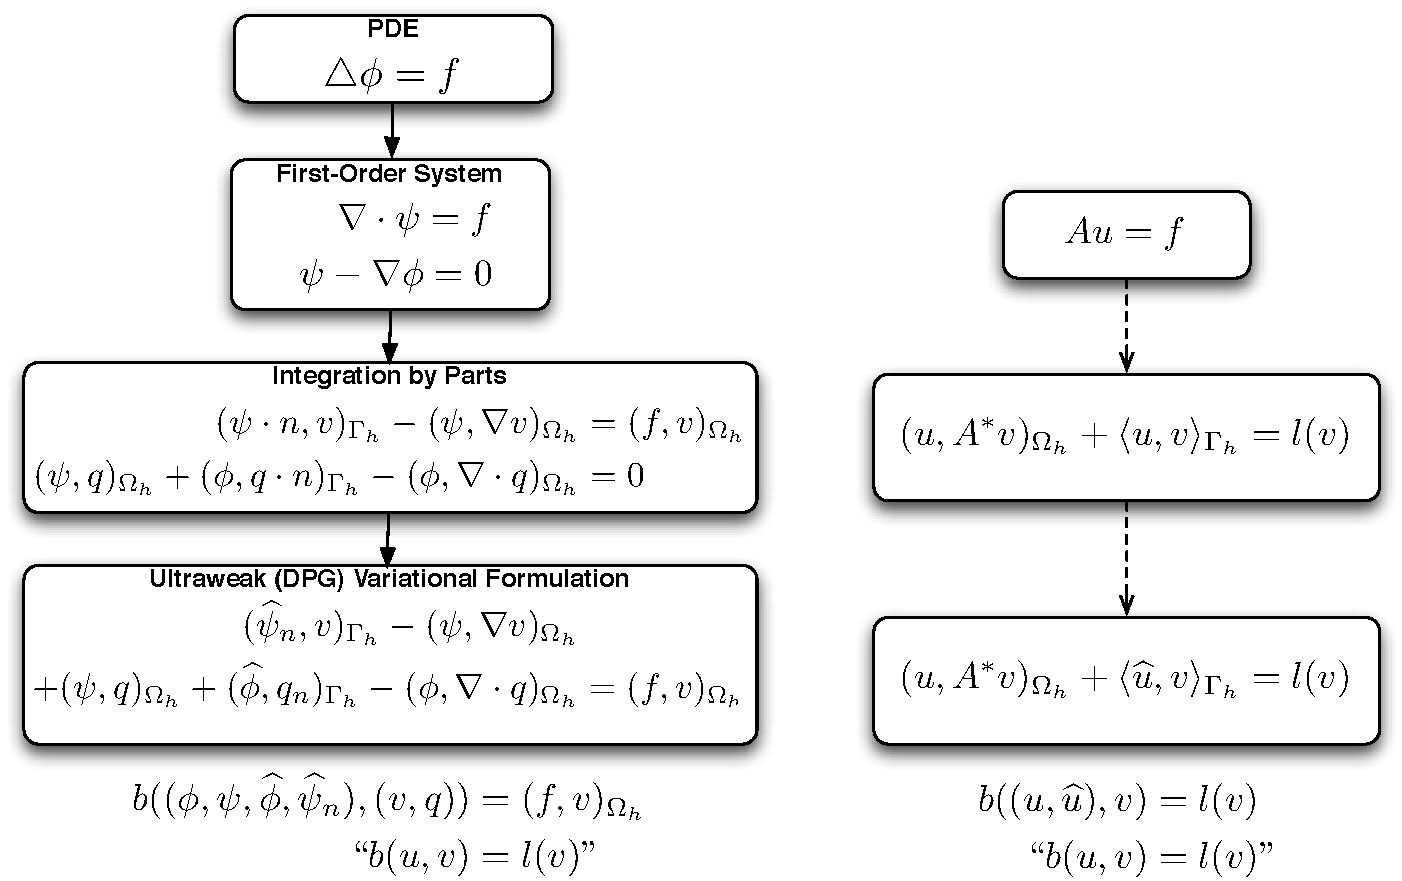
\includegraphics[width=\linewidth]{../figures/DPGFormCartoon}\\
\end{center}
\end{frame}              
%===============================================================================
% Solving with DPG
%===============================================================================
%\begin{frame}                                                                                                                                                                          
%\frametitle{Solving with DPG}
%\begin{center} 
%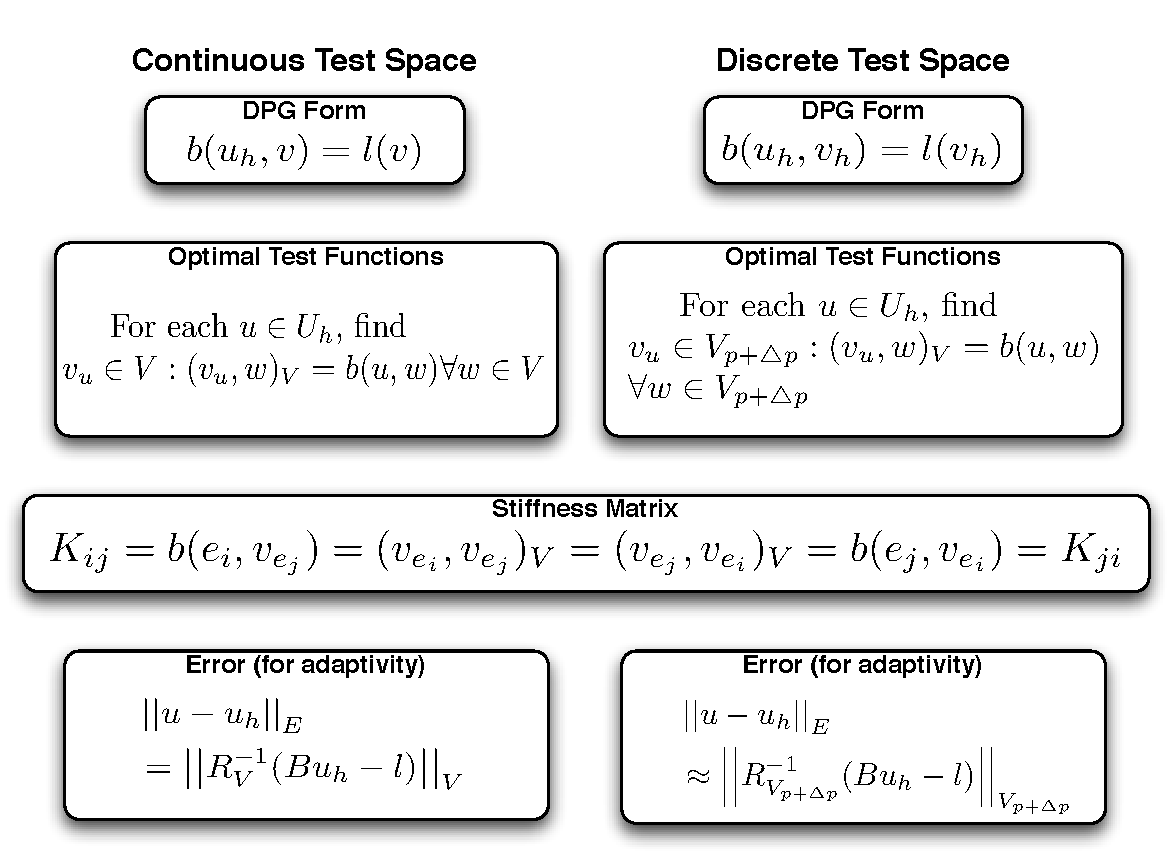
\includegraphics[width=0.9\linewidth]{../figures/DPGSolveCartoonNew}\\
%\end{center}
%\end{frame}

\begin{frame}                                                                                                                                                                          
\frametitle{Solving with DPG}
\begin{itemize}
\item We drive \pecosbold{adaptivity} using an energy norm in which we can precisely determine the error:
\[
\NVRnorm{u-u_{h}}_{E} = \NVRnorm{R_{V}^{-1}\left(Bu_{h} - l \right)}_{V}.
\]
\item In practice, must \pecosbold{approximate} $R_{V}^{-1}$.  We do this by using ``enriched'' test space $V_{p+\Delta p}$.  ($\Delta p=$ 1 or 2, usually.)
\item Test functions belong to a \pecosbold{broken} (element-wise conforming) space.
\item \pecosbold{Discontinuous} test space $\implies$ optimal test functions can be determined element-locally.
\item The system matrix is symmetric-positive definite:
\[
K_{ij} = b(e_{i}, v_{e_{j}}) = (v_{e_{i}}, v_{e_{j}})_{V} = (v_{e_{j}}, v_{e_{i}})_{V} = b(e_{j}, v_{e_{i}}) = K_{ji}
\]
\end{itemize}

\end{frame}

\begin{frame}
\frametitle{Key Features of DPG}\small
\begin{itemize}
\item \pecosbold{guarantees} minimum residual in a norm that depends on the test space, \pecosbold{a free choice}
\item for non-singularly-perturbed, well-posed linear problems, \pecosbold{provably optimal} convergence rates when the ``adjoint graph norm'' is used for the test space
%\item \pecosbold{SPD} stiffness matrix
\item nonlinear problems: so far, apply the linear method to the linearized problem
\item have also derived a method that instead minimizes the nonlinear residual
\end{itemize}
\begin{block}{Adjoint Graph Norm}
For a strong operator $A$ with formal adjoint $A^{*}$, the \pecosbold{adjoint graph norm} on the test space $V$ is given by
\[
\NVRnorm{v}_{\rm graph} = \NVRnorm{v}_{H_{A^{*}}} = \left( \NVRnorm{v}^{2} + \NVRnorm{A^{*}v}^{2}\right)^{1/2}.
\]
\end{block}
\end{frame}

\section{Camellia} % 10-12 slides
\begin{frame}[fragile]
\frametitle{Camellia\footnote{\FootSize \bibentry{RobertsetAl11}}}
\pecosbold{Design Goal}: make DPG research and experimentation as simple as possible, without sacrificing too much by way of performance.
\vspace{3mm}
\begin{center}
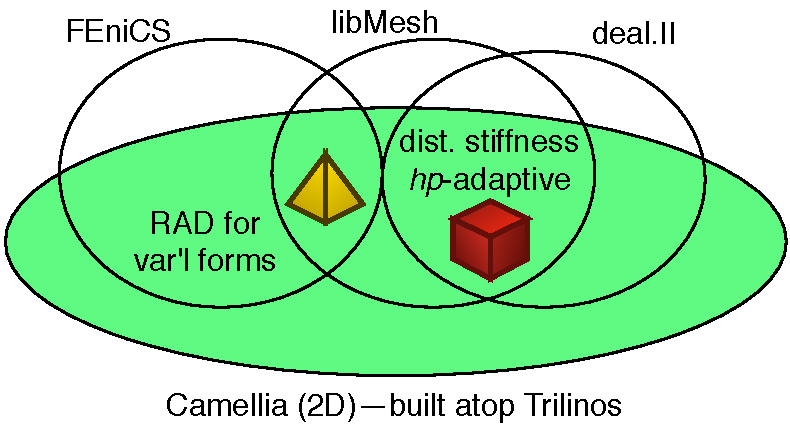
\includegraphics[scale=.65]{../figures/CamelliaVennDiagram.pdf}
\end{center}
\addtocounter{footnote}{1}
\footnotetext{\FootSize \bibentry{TrilinosShortAuthors}}
\end{frame}

\begin{frame}
\frametitle{Camellia: 2011 Design}
\begin{itemize}
\item Camellia defines \pecosbold{abstract classes} for bilinear form, inner product, right-hand side, boundary conditions.
\item User implements problem-specific code through \pecosbold{subclassing}.
\item Allows \pecosbold{automatic} definition of adjoint graph norm.
\end{itemize}

\begin{table}
\begin{center}
\begin{tabular}{| c | c |}
\hline
Implementation & Lines of Code\\
\hline
Stokes bilinear form & 341 \\
Stokes RHS and BCs & 251 \\
Automatic graph norm & 198 \\
\hline
\end{tabular}
\end{center}
\end{table}
\end{frame}

\begin{frame}
\frametitle{Camellia: 2012 Design}
\begin{itemize}
\item Key observation: bilinear form, inner product, and RHS can all be defined using \pecosbold{linear terms} involving the trial and test space variables.
\item We can define a linear term as \code{lt = f * v} where \code{f} is a function and \code{v} is a variable.
\item Functions can depend on spatial coordinates, and may be scalar-, vector-, or tensor-valued.
\item Variables might be operated on by a linear differential operator.
\item Using these as primitives, Camellia allows \pecosbold{declarative} specification of bilinear form, inner product, and RHS.
\end{itemize}
\end{frame}

\begin{frame}[fragile]
\frametitle{Camellia: 2012 Design, Poisson implementation}
Recall our Poisson formulation:
\begin{align*}
\text{``}b(u,v)\text{''} = (\widehat{\psi}_n,v)_{\Gamma_h} - (\vect{\psi}, \nabla v)_{\Omega_h} &\\
+ (\vect{\psi}, \vect{q})_{\Omega_h} + (\widehat{\phi}, \vect{q}  \cdot \vect{n})_{\Gamma_h} - (\phi, \nabla \cdot \vect{q})_{\Omega_h} &= (f,v)_{\Omega_h}.
\end{align*}
\begin{lstlisting}
  VarFactory varFactory; 
  VarPtr v = varFactory.testVar("v", HGRAD);
  VarPtr q = varFactory.testVar("q", HDIV);
    
  VarPtr psi_hat_n = varFactory.fluxVar("\\widehat{\\psi}_n");
  VarPtr phi_hat = varFactory.traceVar("\\widehat{\\phi}");
  VarPtr psi = varFactory.fieldVar("\\psi", VECTOR_L2);
  VarPtr phi = varFactory.fieldVar("\\phi", L2);
\end{lstlisting}

\end{frame}

\begin{frame}[fragile]
\frametitle{Camellia: 2012 Design, Poisson implementation}
Recall our Poisson formulation:
\begin{align*}
\text{``}b(u,v)\text{''} = (\widehat{\psi}_n,v)_{\Gamma_h} - (\vect{\psi}, \nabla v)_{\Omega_h} &\\
+ (\vect{\psi}, \vect{q})_{\Omega_h} + (\widehat{\phi}, \vect{q}  \cdot \vect{n})_{\Gamma_h} - (\phi, \nabla \cdot \vect{q})_{\Omega_h} &= (f,v)_{\Omega_h}.
\end{align*}
\begin{lstlisting}
  BFPtr bf = Teuchos::rcp( new BF(varFactory) );
  
  bf->addTerm(psi_hat_n, v);
  bf->addTerm(-psi, v->grad());
  
  bf->addTerm(psi, q);
  bf->addTerm(phi_hat, q->dot_normal());
  bf->addTerm(-phi, q->div());
\end{lstlisting}

RHS, BCs, and test space norms can be specified in a similar fashion.

\end{frame}

\begin{frame}
\frametitle{Camellia: 2012 vs. 2011 Design, Lines of Code}

\begin{table}[h!b!p!]
\begin{center}
\begin{tabular}{| c | c | c |}
\hline
Implementation & Lines of Code, Old & Lines of Code, New\\
\hline
Stokes bilinear form & 341 & 50 \\
Stokes RHS and BCs & 251 & 90\\
Automatic graph norm & 198 & 36 \\
\hline
\end{tabular}
\end{center}
\end{table}

\begin{block}{Camellia: Future Work}
\begin{itemize}
\item support for curved geometry.
\item minimize the \emph{nonlinear} residual (adds a hessian term).
\item in further future: 1D and 3D mesh support, distributed mesh and solution storage.
\end{itemize}
\end{block}
\end{frame}

%===============================================================================
% THANK YOU
%===============================================================================
\begin{frame}
\frametitle{}
\begin{block}{}
\center{Thank you!} \\
\center{Questions?}\\
\end{block}
\vspace{1cm}
\center{For more info:\\
nroberts@ices.utexas.edu}\\
\end{frame}

\bibliographystyle{plain}
{\scriptsize
\bibliography{../DPG}
}
 
\end{document}
